\documentclass[aspectratio=169]{beamer}
\usepackage{lmodern}
%\usetheme{Madrid}
%\usecolortheme{giantoak}
\newcommand*\oldmacro{}
\let\oldmacro\insertshorttitle
\renewcommand*\insertshorttitle{\oldmacro\hfill\insertframenumber\,/\,\inserttotalframenumber}
\usepackage[framemethod=tikz]{mdframed}

%\usepackage{beamerthemesplit}
\usepackage{textpos}
\usepackage{pgf}
%\logo{\pgfputat{\pgfxy(0,-.4)}{\pgfbox[right,base]{\includegraphics[height=1.0cm]{logo.jpg}}}}
%\newcommand{\nologo}{\setbeamertemplate{logo}{}}
\usepackage{booktabs}
\usepackage{graphicx}
\theoremstyle{principle}
\newtheorem*{principle}{Design Principle}


\titlegraphic{\includegraphics[width=1.0\paperwidth]{cool-wind-800px.jpg}}

\title{Intro to Data and Descriptive Statistics}
%\author[Jeremy Kedziora]{Wind Data Science Team\\
%\small{Uptake}}
\date{}

\begin{document}

%{
%%\nologo
%\begin{frame}
%    \maketitle
%\end{frame}
%}
%pages 1-7, 8-9, 14-15.


{
%  \usebackgroundtemplate{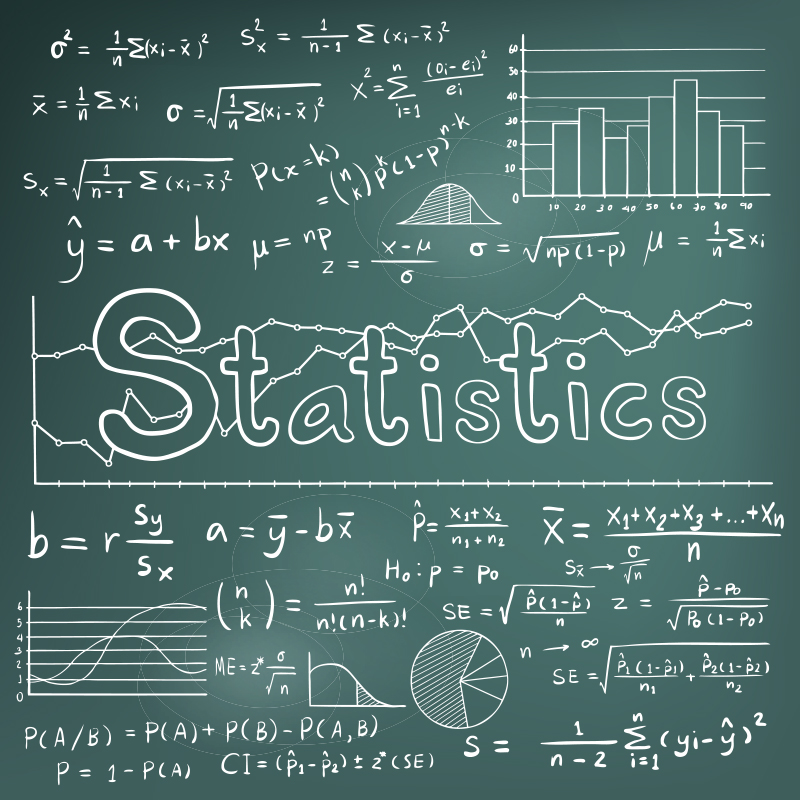
\includegraphics[width=1.0\paperwidth]{statistics-review.jpg}}
  \usebackgroundtemplate{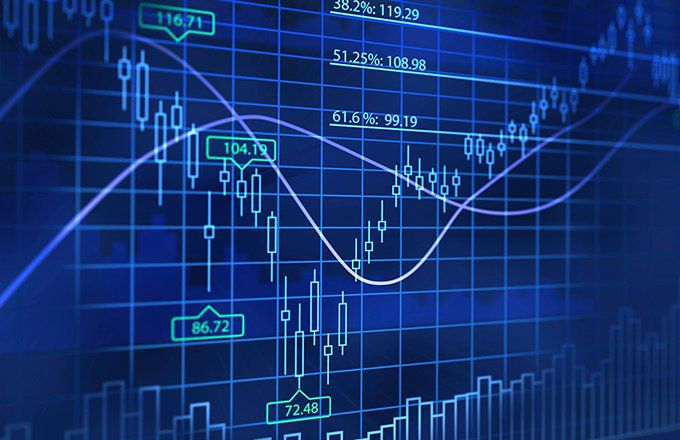
\includegraphics[scale=0.7]{descriptive_stats.jpg}}
  \begin{frame}[plain]
  
\begin{mdframed}[tikzsetting={draw=white,fill=white,fill opacity=0.6,draw opacity=0.4,
               line width=0pt},backgroundcolor=none,leftmargin=20,
               rightmargin=20,innertopmargin=4pt]
\begin{center}
\Huge \textbf{Intro to Data and Descriptive Statistics}
\end{center}
\end{mdframed}

  \end{frame}
}

%@@@@@@@@@@@@@@@@@@@@@@@@@@@@@@@@@@@@@@@@@@@@@@@@@
\begin{frame}
\frametitle{Today:}

\begin{itemize}
\item What are different types of data?
\bigskip
\bigskip
\item What are descriptive statistics and what job do they do?
\bigskip
\bigskip
\item Which descriptive statistics are appropriate for which type of data?
\end{itemize}

\end{frame}

%@@@@@@@@@@@@@@@@@@@@@@@@@@@@@@@@@@@@@@@@@@@@@@@@@
\begin{frame}
\frametitle{Data Types: the `Levels of Measurement'} 
\begin{itemize}
\item \textbf{Nominal};
\begin{itemize}
\item Qualitative classification of different objects by names -- measures membership;
\item Examples: Gender, nationality, zip code, eye color, error code;
\item[]
\end{itemize}

\item \textbf{Ordinal};
\begin{itemize}
\item Categories with a natural ordering, but no well-defined scale -- measures rank;
\item Examples: Party membership, polling agreement (Likert) scales, ed level, class;
\item[]
\end{itemize}

\item \textbf{Interval};
\begin{itemize}
\item Difference btwn units on scale is constant, but no zero point -- measures exact difference;
\item Examples: Time of day, date, temperature (F or C), test scores, IQ;
\item[]
\end{itemize}

\item \textbf{Ratio};
\begin{itemize}
\item Difference btwn units on scale is constant/has a zero point -- measures exact difference $+$;
\item Examples: Height and weight, earnings, military spending, tax rate, temperature (K).
\item[]
\end{itemize}
\end{itemize}
\end{frame}

%@@@@@@@@@@@@@@@@@@@@@@@@@@@@@@@@@@@@@@@@@@@@@@@@@
\begin{frame}
\frametitle{What are descriptive statistics?!}
\begin{itemize}
\item In general, two kinds of statistics:
\begin{itemize}
\item \textbf{Descriptive Statistics} -- what we'll talk about today;
\item \textbf{Inferential Statistics} -- what we'll spend much of the rest of the semester on;
\end{itemize}
\bigskip
\bigskip
\item Typically, descriptive statistics are always reported even if main focus is on something more sophisticated.
\end{itemize}
\end{frame}

%@@@@@@@@@@@@@@@@@@@@@@@@@@@@@@@@@@@@@@@@@@@@@@@@@
\begin{frame}
\frametitle{What are descriptive statistics: key terms}
\begin{itemize}
\item \textbf{Population}: a `complete' group of $N$ objects, items, entities, or events of interest -- e.g. all adults living in the US;
\bigskip
\item \textbf{Sample}: a selected subset of $n$ individuals from a population -- e.g. 5,000 US adults appearing in a poll;
\bigskip
\item \textbf{Summary Statistic}: a summary of the information in a set of observations -- e.g. mean, median, mode, etc.;
\bigskip
\item \textbf{Parametric}: derived from a probability distribution -- e.g. a $z$-score is related to a normal distribution;
\bigskip
\item \textbf{Nonparametric}: NOT derived from a probability distribution -- e.g. descriptive statistics, histograms, etc.;
\bigskip
\item \textbf{Univariate}: dealing with a single variable;
\bigskip
\item \textbf{Multivariate}: dealing with relationships between several variables;
\end{itemize}
\end{frame}

%@@@@@@@@@@@@@@@@@@@@@@@@@@@@@@@@@@@@@@@@@@@@@@@@@
\begin{frame}
\frametitle{What job do they do?}

\begin{columns}
\begin{column}{0.5\textwidth}

\begin{itemize}
\item The main job of descriptive statistics is to \textbf{summarize} the information in a \textbf{sample};
\begin{itemize}
\item ...describe the data in the sample;
\item ...assess data quality (e.g. variation, correlation btwn variables, etc.);
\item ...support later inferential analysis;
\end{itemize}
\bigskip
\bigskip
\item The main job of inferential statistics is to \textbf{learn} about the \textbf{population} that the sample comes from.
\end{itemize}

\end{column}
\begin{column}{0.5\textwidth}
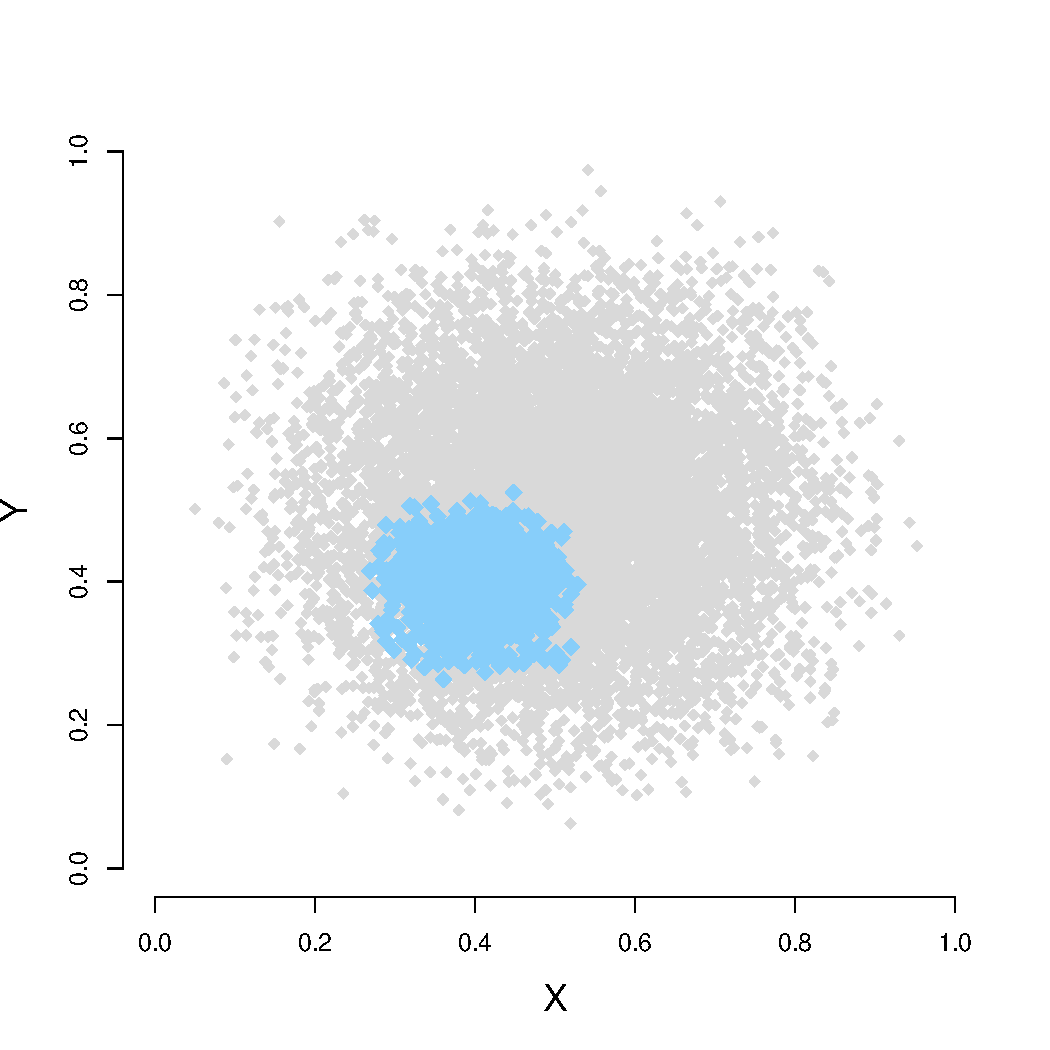
\includegraphics[scale=0.4]{point_cloud.pdf}
\end{column}
\end{columns}

\end{frame}

%@@@@@@@@@@@@@@@@@@@@@@@@@@@@@@@@@@@@@@@@@@@@@@@@@
\begin{frame}
\begin{center}
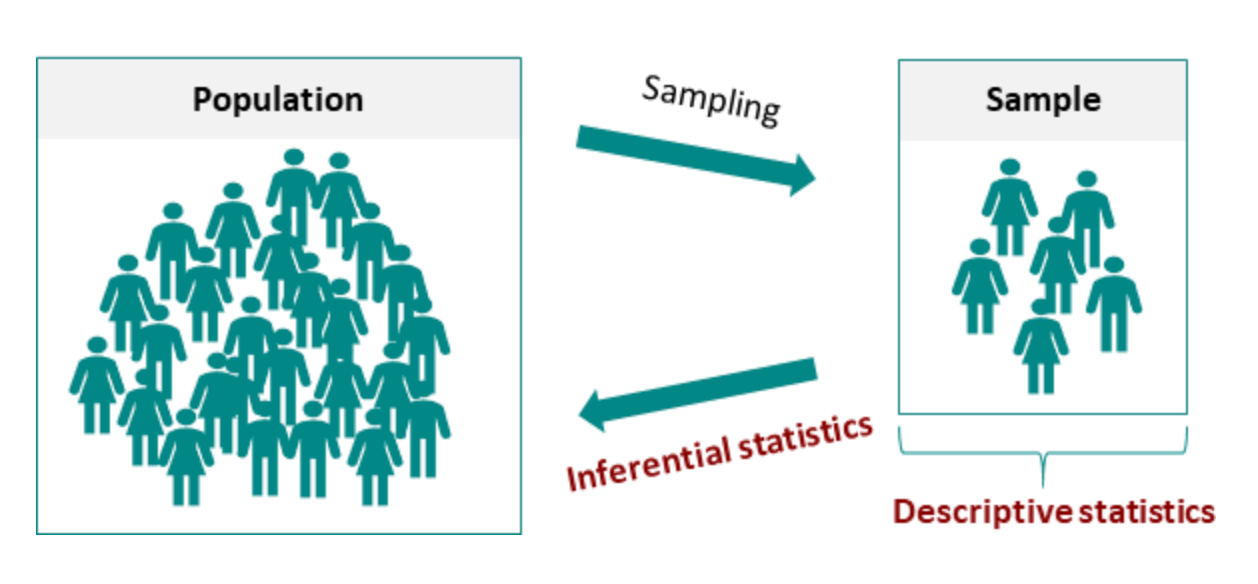
\includegraphics[scale=0.6]{descriptive_inference.png}
\end{center}

\end{frame}

%@@@@@@@@@@@@@@@@@@@@@@@@@@@@@@@@@@@@@@@@@@@@@@@@@
\begin{frame}
\frametitle{Measures of Central Tendency (for dataset $x$: $0, 1, 4, 4, 5, 5, 7, 7, 7, 9, 9$)}
\begin{itemize}

\item \textbf{Mode} -- the \textbf{sample} mode is written as $\overline{x}_{mode}$ and is the element that occurs most often in the sample.  In our example $\overline{x}_{mode} = 7$.

\item[] \color{white}\textbf{Median} --  the \textbf{sample} median is written as $\overline{x}_{med}$:
\begin{align*}
\overline{x}_{med} = \left\{\begin{array}{ll}
x_{(n+1)/2}&\mbox{if }n\mbox{ is odd}\\
x_{(n/2)} + x_{(n/2)+1}&\mbox{if }n\mbox{ is even}
\end{array}\right.\Longrightarrow \overline{x}_{med} = x_{(11 + 1)/2} = x_6 = 5.
\end{align*}

\item[] \color{white} \textbf{Arithmetic mean} -- the \textbf{sample} mean is written as $\overline{x}$:
\bigskip
\begin{align*}
\overline{x} &= \frac{1}{n}\left(\sum_{i=1}^nx_i\right) \Longrightarrow \frac{0 + 1 + 4 + 4 + 5 + 5 +7 + 7 + 7 + 9 + 9}{11}\approx 5.273.
\end{align*}

\item[] \color{white} \textbf{Midrange} -- the \textbf{sample} midrange is written as $\overline{x}_{mid}$:
\begin{align*}
\overline{x}_{mid} = \frac{\max\{x\} + \min\{x\}}{2}\Longrightarrow\overline{x}_{mid} = \frac{9 + 0}{2} = 4.5.
\end{align*}

\end{itemize}
\end{frame}

%@@@@@@@@@@@@@@@@@@@@@@@@@@@@@@@@@@@@@@@@@@@@@@@@@
\begin{frame}
\frametitle{Measures of Central Tendency (for dataset $x$: $0, 1, 4, 4, 5, 5, 7, 7, 7, 9, 9$)}
\begin{itemize}

\item[] \color{white} \textbf{Mode} -- the \textbf{sample} mode is written as $\overline{x}_{mode}$ and is the element that occurs most often in the sample.  In our example $\overline{x}_{mode} = 7$.

\item \color{black}\textbf{Median} --  the \textbf{sample} median is written as $\overline{x}_{med}$:
\begin{align*}
\overline{x}_{med} = \left\{\begin{array}{ll}
x_{(n+1)/2}&\mbox{if }n\mbox{ is odd}\\
x_{(n/2)} + x_{(n/2)+1}&\mbox{if }n\mbox{ is even}
\end{array}\right.\Longrightarrow \overline{x}_{med} = x_{(11 + 1)/2} = x_6 = 5.
\end{align*}

\item[] \color{white} \textbf{Arithmetic mean} -- the \textbf{sample} mean is written as $\overline{x}$:
\bigskip
\begin{align*}
\overline{x} &= \frac{1}{n}\left(\sum_{i=1}^nx_i\right) \Longrightarrow \frac{0 + 1 + 4 + 4 + 5 + 5 +7 + 7 + 7 + 9 + 9}{11}\approx 5.273.
\end{align*}

\item[] \color{white} \textbf{Midrange} -- the \textbf{sample} midrange is written as $\overline{x}_{mid}$:
\begin{align*}
\overline{x}_{mid} = \frac{\max\{x\} + \min\{x\}}{2}\Longrightarrow\overline{x}_{mid} = \frac{9 + 0}{2} = 4.5.
\end{align*}

\end{itemize}
\end{frame}

%@@@@@@@@@@@@@@@@@@@@@@@@@@@@@@@@@@@@@@@@@@@@@@@@@
\begin{frame}
\frametitle{Measures of Central Tendency (for dataset $x$: $0, 1, 4, 4, 5, 5, 7, 7, 7, 9, 9$)}
\begin{itemize}

\item[] \color{white} \textbf{Mode} -- the \textbf{sample} mode is written as $\overline{x}_{mode}$ and is the element that occurs most often in the sample.  In our example $\overline{x}_{mode} = 7$.

\item[] \color{white}\textbf{Median} --  the \textbf{sample} median is written as $\overline{x}_{med}$:
\begin{align*}
\overline{x}_{med} = \left\{\begin{array}{ll}
x_{(n+1)/2}&\mbox{if }n\mbox{ is odd}\\
x_{(n/2)} + x_{(n/2)+1}&\mbox{if }n\mbox{ is even}
\end{array}\right.\Longrightarrow \overline{x}_{med} = x_{(11 + 1)/2} = x_6 = 5.
\end{align*}

\item \color{black} \textbf{Arithmetic mean} -- the \textbf{sample} mean is written as $\overline{x}$:
\bigskip
\begin{align*}
\overline{x} &= \frac{1}{n}\left(\sum_{i=1}^nx_i\right) \Longrightarrow \frac{0 + 1 + 4 + 4 + 5 + 5 +7 + 7 + 7 + 9 + 9}{11}\approx 5.273.
\end{align*}

\item[] \color{white} \textbf{Midrange} -- the \textbf{sample} midrange is written as $\overline{x}_{mid}$:
\begin{align*}
\overline{x}_{mid} = \frac{\max\{x\} + \min\{x\}}{2}\Longrightarrow\overline{x}_{mid} = \frac{9 + 0}{2} = 4.5.
\end{align*}

\end{itemize}
\end{frame}

%@@@@@@@@@@@@@@@@@@@@@@@@@@@@@@@@@@@@@@@@@@@@@@@@@
\begin{frame}
\frametitle{Measures of Central Tendency (for dataset $x$: $0, 1, 4, 4, 5, 5, 7, 7, 7, 9, 9$)}
\begin{itemize}

\item[] \color{white}\textbf{Mode} -- the \textbf{sample} mode is written as $\overline{x}_{mode}$ and is the element that occurs most often in the sample.  In our example $\overline{x}_{mode} = 7$.

\item[] \color{white}\textbf{Median} --  the \textbf{sample} median is written as $\overline{x}_{med}$:
\begin{align*}
\overline{x}_{med} = \left\{\begin{array}{ll}
x_{(n+1)/2}&\mbox{if }n\mbox{ is odd}\\
x_{(n/2)} + x_{(n/2)+1}&\mbox{if }n\mbox{ is even}
\end{array}\right.\Longrightarrow \overline{x}_{med} = x_{(11 + 1)/2} = x_6 = 5.
\end{align*}

\item[] \color{white} \textbf{Arithmetic mean} -- the \textbf{sample} mean is written as $\overline{x}$:
\bigskip
\begin{align*}
\overline{x} &= \frac{1}{n}\left(\sum_{i=1}^nx_i\right) \Longrightarrow \frac{0 + 1 + 4 + 4 + 5 + 5 +7 + 7 + 7 + 9 + 9}{11}\approx 5.273.
\end{align*}

\item \color{black} \textbf{Midrange} -- the \textbf{sample} midrange is written as $\overline{x}_{mid}$:
\begin{align*}
\overline{x}_{mid} = \frac{\max\{x\} + \min\{x\}}{2}\Longrightarrow\overline{x}_{mid} = \frac{9 + 0}{2} = 4.5.
\end{align*}

\end{itemize}
\end{frame}

%@@@@@@@@@@@@@@@@@@@@@@@@@@@@@@@@@@@@@@@@@@@@@@@@@
\begin{frame}
\frametitle{Measures of Variability (for dataset $x$: $0, 1, 4, 4, 5, 5, 7, 7, 7, 9, 9$)}
\begin{itemize}

\item \textbf{Range} -- written as $\sigma_{max}$, the distance between the min and max: 
\begin{align*}
\sigma_{max} = \max\{x\} - \min\{x\} \Longrightarrow 9 - 0 = 9.
\end{align*}

\item[]\color{white} \textbf{Variation ratio} -- written as $\sigma_{vr}$, the proportion of cases NOT in the modal category:
\begin{align*}
\sigma_{vr} = 1 - \frac{f_m}{n}\Longrightarrow 1 - \frac{3}{11} \approx 0.727, \mbox{where  }f_m =\mbox{ number of cases IN the modal category}.
\end{align*}

\item[]\color{white} \textbf{Standard deviation/Variance} -- written as $\sigma$, the sum of squared distance from mean:
\begin{align*}
\sigma = \sqrt{\frac{1}{n}\sum_{i=1}^n(x_i - \overline{x})^2} = \sqrt{\frac{(0 - 5.273)^2 + (1 - 5.273)^2 + \hdots + (9 - 5.273)^2}{11}}\approx 2.799.
\end{align*}

\end{itemize}
\end{frame}

%@@@@@@@@@@@@@@@@@@@@@@@@@@@@@@@@@@@@@@@@@@@@@@@@@
\begin{frame}
\frametitle{Measures of Variability (for dataset $x$: $0, 1, 4, 4, 5, 5, 7, 7, 7, 9, 9$)}
\begin{itemize}

\item[]\color{white} \textbf{Range} -- written as $\sigma_{max}$, the distance between the min and max: 
\begin{align*}
\sigma_{max} = \max\{x\} - \min\{x\} \Longrightarrow 9 - 0 = 9.
\end{align*}

\item\color{black} \textbf{Variation ratio} -- written as $\sigma_{vr}$, the proportion of cases NOT in the modal category:
\begin{align*}
\sigma_{vr} = 1 - \frac{f_m}{n}\Longrightarrow 1 - \frac{3}{11} \approx 0.727, \mbox{where  }f_m =\mbox{ \# of cases IN the modal category}.
\end{align*}

\item[]\color{white} \textbf{Standard deviation/Variance} -- written as $\sigma$, the sum of squared distance from mean:
\begin{align*}
\sigma = \sqrt{\frac{1}{n}\sum_{i=1}^n(x_i - \overline{x})^2} = \sqrt{\frac{(0 - 5.273)^2 + (1 - 5.273)^2 + \hdots + (9 - 5.273)^2}{11}}\approx 2.799.
\end{align*}

\end{itemize}
\end{frame}

%@@@@@@@@@@@@@@@@@@@@@@@@@@@@@@@@@@@@@@@@@@@@@@@@@
\begin{frame}
\frametitle{Measures of Variability (for dataset $x$: $0, 1, 4, 4, 5, 5, 7, 7, 7, 9, 9$)}
\begin{itemize}

\item[]\color{white} \textbf{Range} -- written as $\sigma_{max}$, the distance between the min and max: 
\begin{align*}
\sigma_{max} = \max\{x\} - \min\{x\} \Longrightarrow 9 - 0 = 9.
\end{align*}

\item[]\color{white} \textbf{Variation ratio} -- written as $\sigma_{vr}$, the proportion of cases NOT in the modal category:
\begin{align*}
\sigma_{vr} = 1 - \frac{f_m}{n}\Longrightarrow 1 - \frac{3}{11} \approx 0.727, \mbox{where  }f_m =\mbox{ number of cases IN the modal category}.
\end{align*}

\item \color{black} \textbf{Standard deviation/Variance} -- written as $\sigma$, the sum of squared distance from mean:
\begin{align*}
\sigma = \sqrt{\frac{1}{n}\sum_{i=1}^n(x_i - \overline{x})^2} = \sqrt{\frac{(0 - 5.273)^2 + (1 - 5.273)^2 + \hdots + (9 - 5.273)^2}{11}}\approx 2.799.
\end{align*}

\end{itemize}
\end{frame}






%@@@@@@@@@@@@@@@@@@@@@@@@@@@@@@@@@@@@@@@@@@@@@@@@@
\begin{frame}
\begin{center}
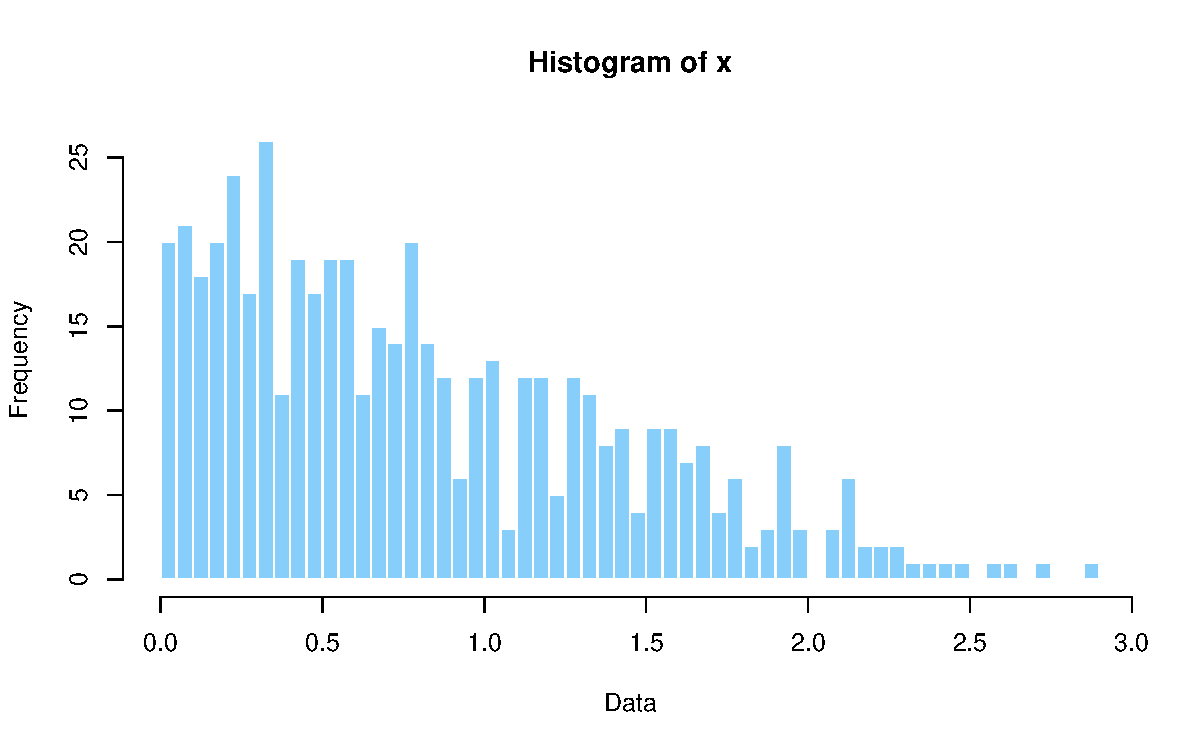
\includegraphics[scale=0.65]{histogram.pdf}
\end{center}
\end{frame}

%@@@@@@@@@@@@@@@@@@@@@@@@@@@@@@@@@@@@@@@@@@@@@@@@@
\begin{frame}
\begin{center}
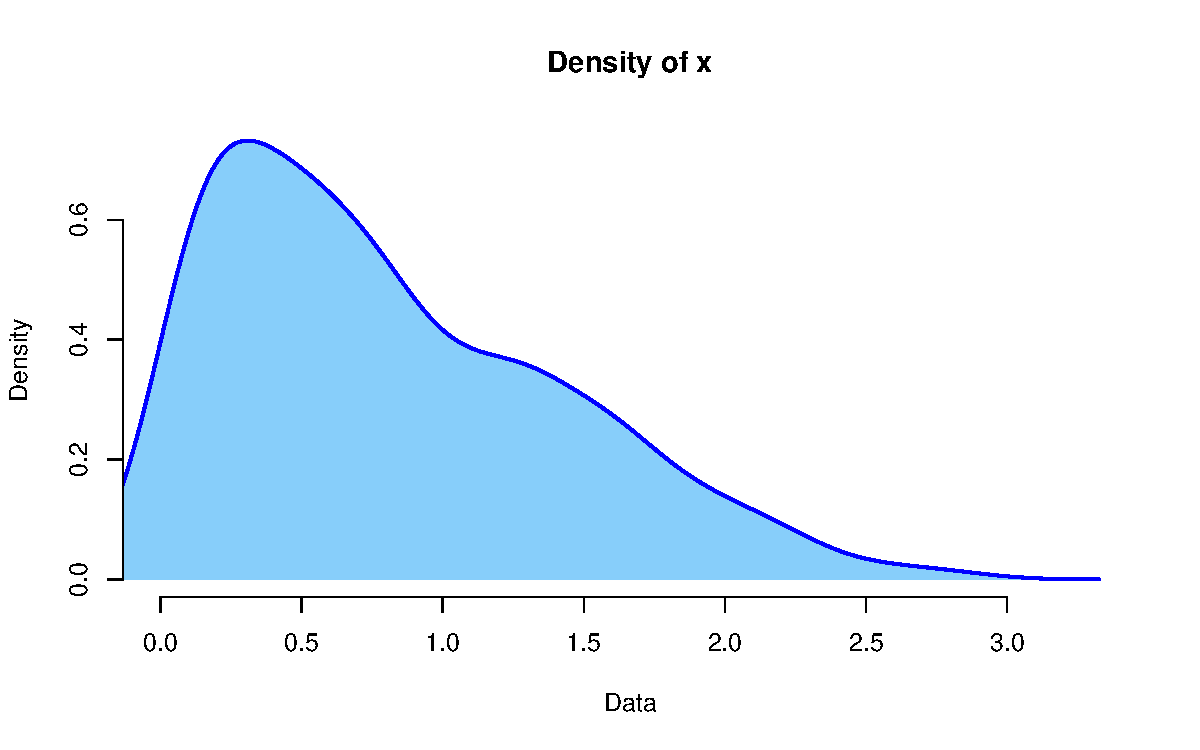
\includegraphics[scale=0.65]{density.pdf}
\end{center}
\end{frame}

%@@@@@@@@@@@@@@@@@@@@@@@@@@@@@@@@@@@@@@@@@@@@@@@@@
\begin{frame}
\begin{center}
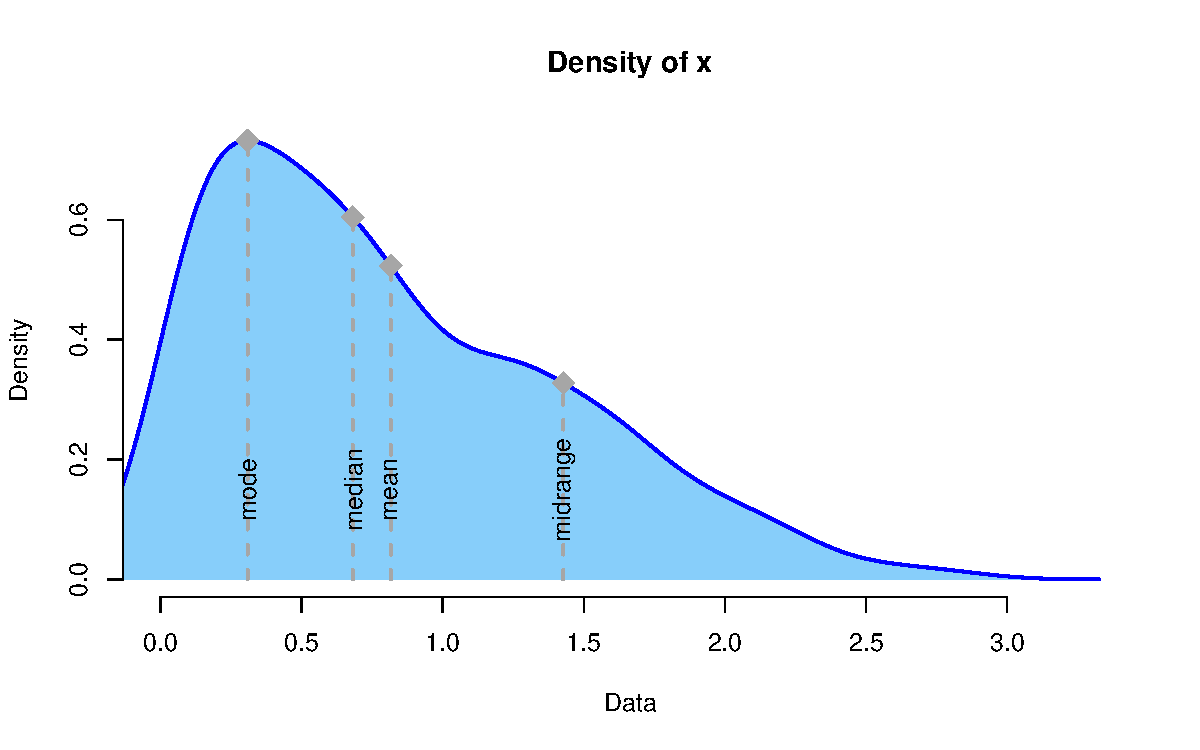
\includegraphics[scale=0.65]{density_w_centrals.pdf}
\end{center}
\end{frame}

%%@@@@@@@@@@@@@@@@@@@@@@@@@@@@@@@@@@@@@@@@@@@@@@@@@
%\begin{frame}
%\frametitle{More than one variable}
%\begin{itemize}
%\item Blar;
%\bigskip
%\bigskip
%\item Blar;
%\bigskip
%\bigskip
%\item Blar;
%\bigskip
%\bigskip
%\item Blar;
%\end{itemize}
%\end{frame}

%@@@@@@@@@@@@@@@@@@@@@@@@@@@@@@@@@@@@@@@@@@@@@@@@@
\begin{frame}
\frametitle{Data Types: the `Levels of Measurement'} 
\begin{itemize}
\item \textbf{Nominal};
\begin{itemize}
\item Qualitative classification of different objects by names -- measures membership;
\item Examples: Gender, nationality, zip code, eye color, error code;
\item Appropriate: equality, mode, Variation ratio;
\end{itemize}
\item \textbf{Ordinal};
\begin{itemize}
\item Categories with a natural ordering, but no well-defined scale -- measures rank;
\item Examples: Party membership, polling agreement (Likert) scales, ed level, class;
\item Appropriate: above plus $>$ and $<$, median, range;
\end{itemize}
\item \textbf{Interval};
\begin{itemize}
\item Difference btwn units on scale is constant, but no zero point -- measures exact difference;
\item Examples: Time of day, date, temperature (F or C), test scores, IQ;
\item Appropriate: above plus $+$ and $-$, mean, standard deviation;
\end{itemize}
\item \textbf{Ratio};
\begin{itemize}
\item Difference btwn units on scale is constant/has a zero point -- measures exact difference $+$;
\item Examples: Height and weight, earnings, military spending, tax rate, temperature (K).
\item Appropriate: above plus $*$ and $/$
\end{itemize}
\end{itemize}
\end{frame}

%@@@@@@@@@@@@@@@@@@@@@@@@@@@@@@@@@@@@@@@@@@@@@@@@@
\begin{frame}
\frametitle{Example: Gender Wage Gap}

\begin{columns}
\begin{column}{0.5\textwidth}

\begin{itemize}
\item Lots of progress -- more women in labor market with higher education than ever;
\bigskip
\item Refers to the earnings difference between women and men:
\begin{itemize}
\item Women consistently earn less than men in US;
\item But how to measure just how much less?
\item ...and what drives the gap???
\end{itemize}
\bigskip
\item \href{https://www.americanprogress.org/article/quick-facts-gender-wage-gap/}{Simple descriptive statistics}:
\begin{itemize}
\item Compute median annual earnings for women and men working full time;
\item Take the ratio.
\item[] \color{white} Is this enough?
\end{itemize}
\end{itemize}

\end{column}
\begin{column}{0.5\textwidth}
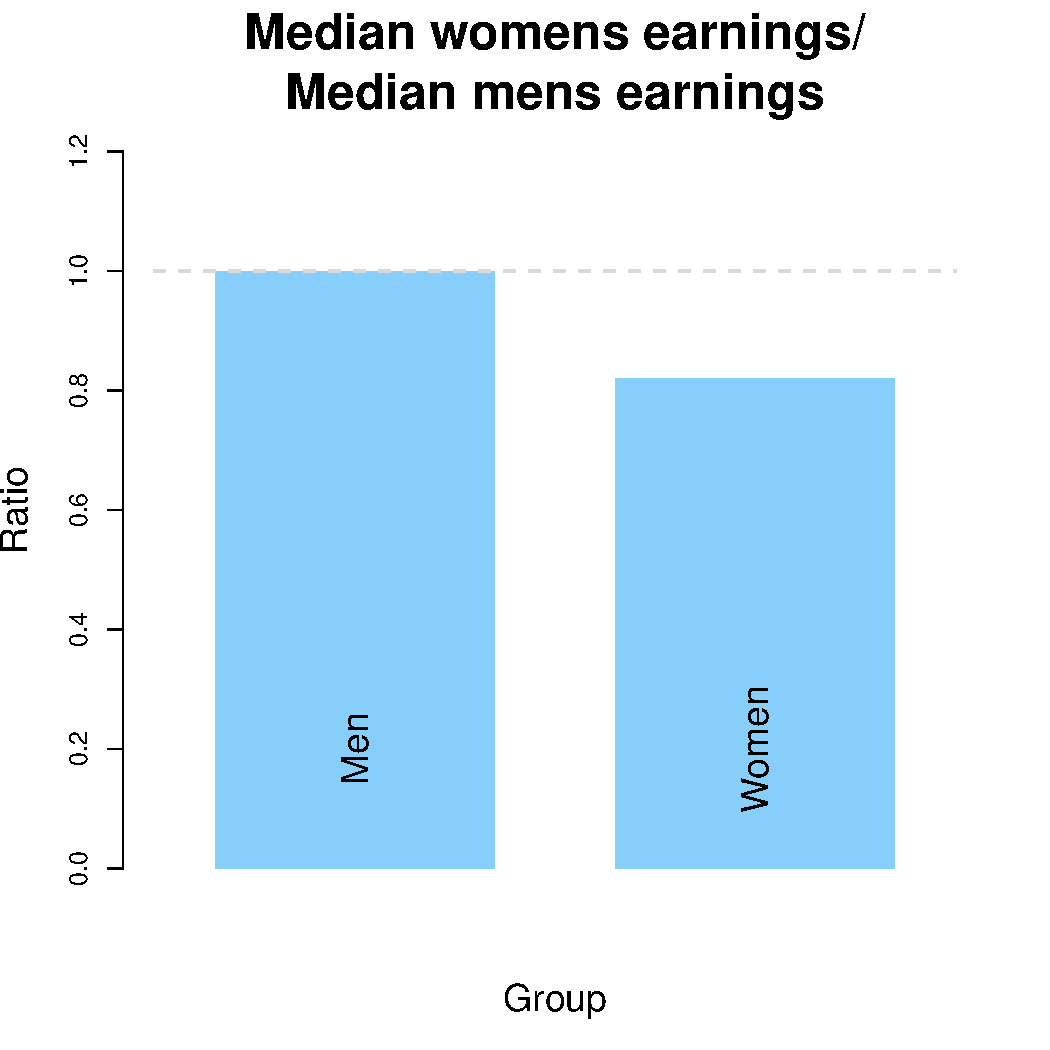
\includegraphics[scale=0.4]{gender_wage_gap.pdf}
\end{column}
\end{columns}

\end{frame}

%@@@@@@@@@@@@@@@@@@@@@@@@@@@@@@@@@@@@@@@@@@@@@@@@@
\begin{frame}
\frametitle{Example: Gender Wage Gap}

\begin{columns}
\begin{column}{0.5\textwidth}

\begin{itemize}
\item Lots of progress -- more women in labor market with higher education than ever;
\bigskip
\item Refers to the earnings difference between women and men:
\begin{itemize}
\item Women consistently earn less than men in US;
\item But how to measure just how much less?
\item ...and what drives the gap???
\end{itemize}
\bigskip
\item \href{https://www.americanprogress.org/article/quick-facts-gender-wage-gap/}{Simple descriptive statistics}:
\begin{itemize}
\item Compute median annual earnings for women and men working full time;
\item Take the ratio.
\item Is this enough?
\end{itemize}
\end{itemize}

\end{column}
\begin{column}{0.5\textwidth}
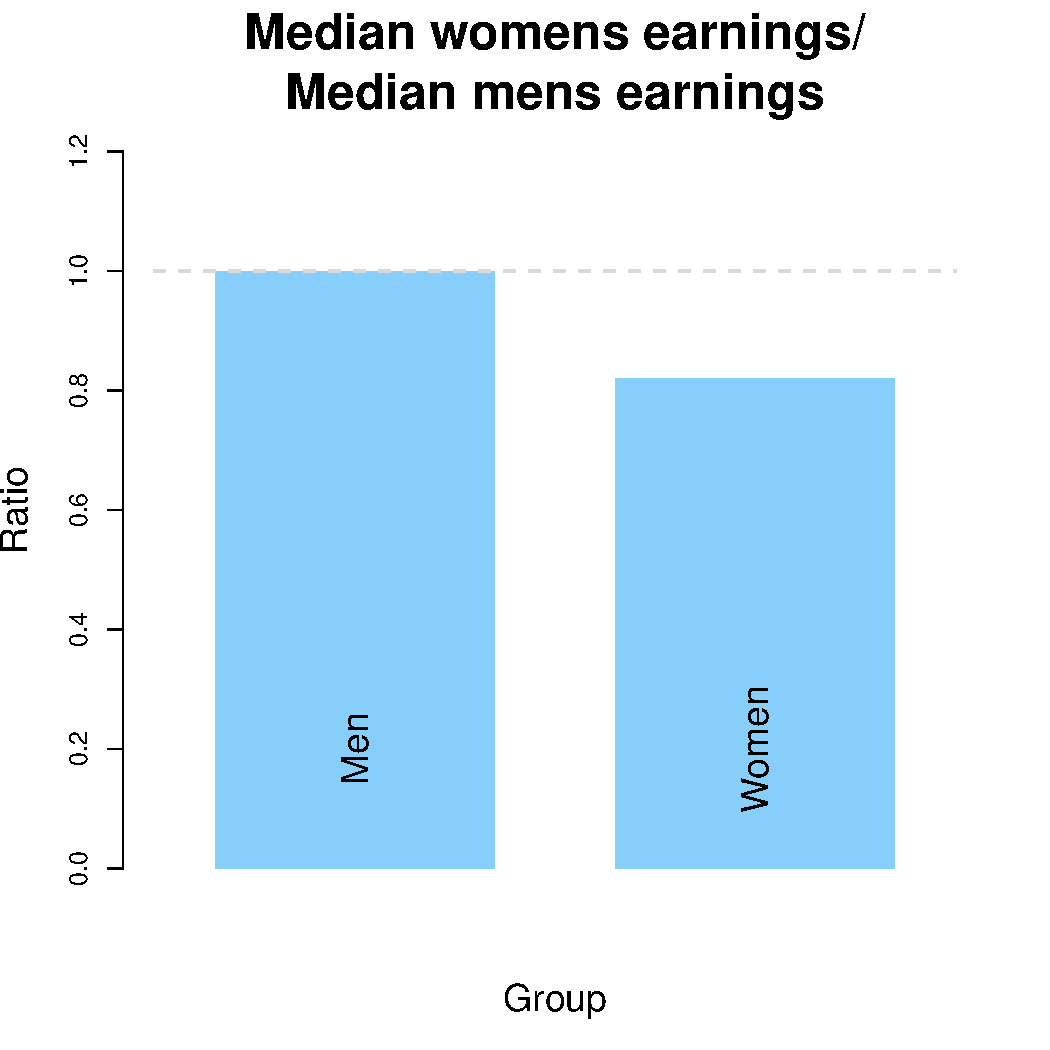
\includegraphics[scale=0.4]{gender_wage_gap.pdf}
\end{column}
\end{columns}

\end{frame}

%@@@@@@@@@@@@@@@@@@@@@@@@@@@@@@@@@@@@@@@@@@@@@@@@@
\begin{frame}
\frametitle{Example: Gender Wage Gap}

\begin{columns}
\begin{column}{0.5\textwidth}

\begin{itemize}
\item Lots of progress -- more women in labor market with higher education than ever;
\bigskip
\item Refers to the earnings difference between women and men:
\begin{itemize}
\item Women consistently earn less than men in US;
\item But how to measure just how much less?
\item ...and what drives the gap???
\end{itemize}
\bigskip
\item \href{https://www.americanprogress.org/article/quick-facts-gender-wage-gap/}{Simple descriptive statistics}:
\begin{itemize}
\item Compute median annual earnings for women and men working full time;
\item Take the ratio.
\item Is this enough?  NO!!!
\end{itemize}
\end{itemize}

\end{column}
\begin{column}{0.5\textwidth}
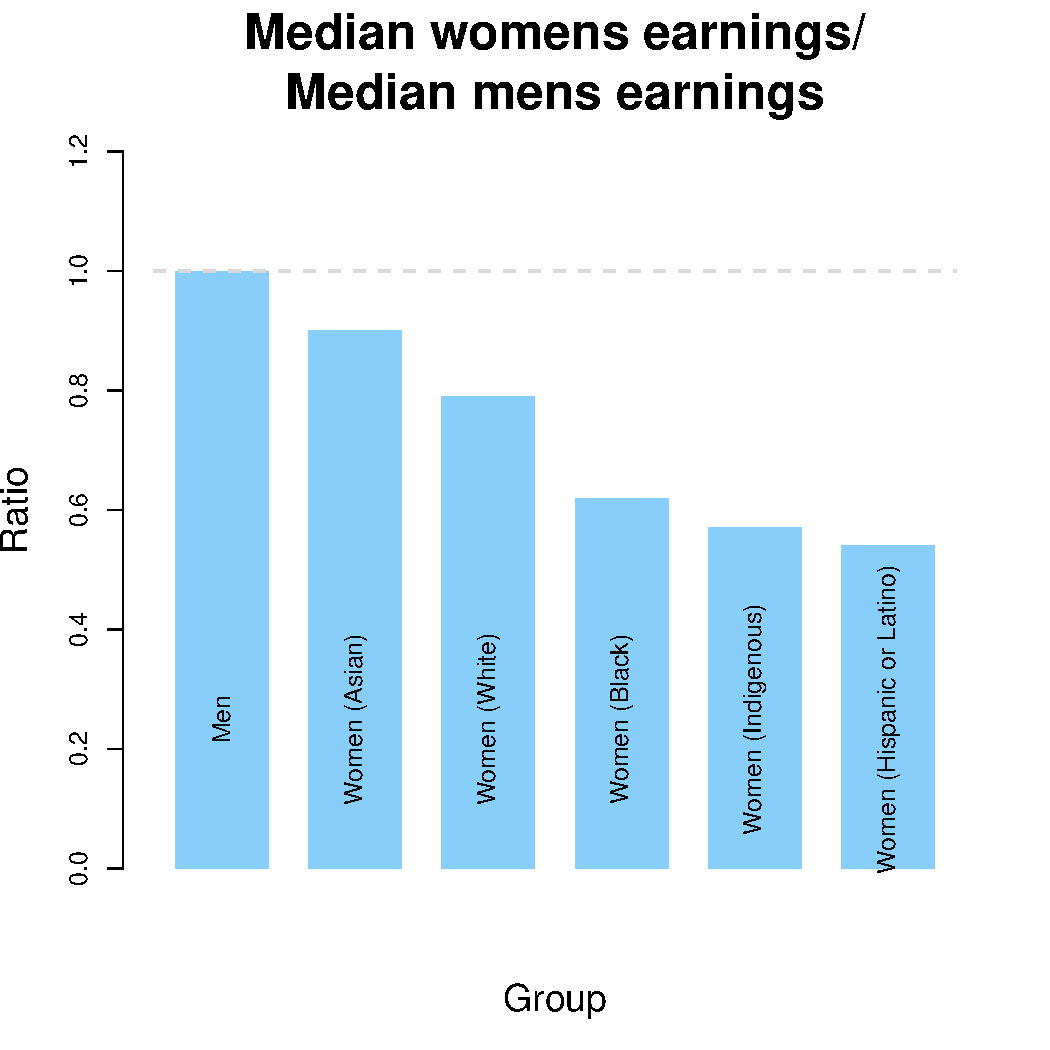
\includegraphics[scale=0.4]{gender_wage_gap_DA.pdf}
\end{column}
\end{columns}

\end{frame}

%hours worked, experience, education, sector, etc.

%@@@@@@@@@@@@@@@@@@@@@@@@@@@@@@@@@@@@@@@@@@@@@@@@@
\begin{frame}

\begin{center}
\Huge\textbf{Why should we care?}\\
\bigskip
\bigskip
\large Using the right descriptive statistics for your data is a good and EASY first pass.\\
\end{center}

\end{frame}



\end{document}






